\item \textbf{Gas Mileage  [27 pts]}.  For a particular model of car, the miles per gallon (mpg) rating obtained for highway driving follows a Normal distribution with mean 28.5 mpg and standard deviation 1.4 mpg.  Use this information to answer the following questions.

\begin{enumerate}
\item \textbf{[3 pts]}What is the probability a car will obtain a miles per gallon rating for highway driving greater than 32 mpg? Answer this question by completing parts (i) and (ii). 

\begin{enumerate}
\item \textbf{[1 pt]}Provide the z-score corresponding to the above statement. \\
 \red{$z = \frac{x-\mu}{\sigma}=\frac{32-28.5}{1.4}=2.50$}
\item \textbf{[2 pts]} Based on your answer in (i), what is the probability a car will obtain a miles per gallon rating for highway driving greater than 32 mpg? \\
\begin{center}
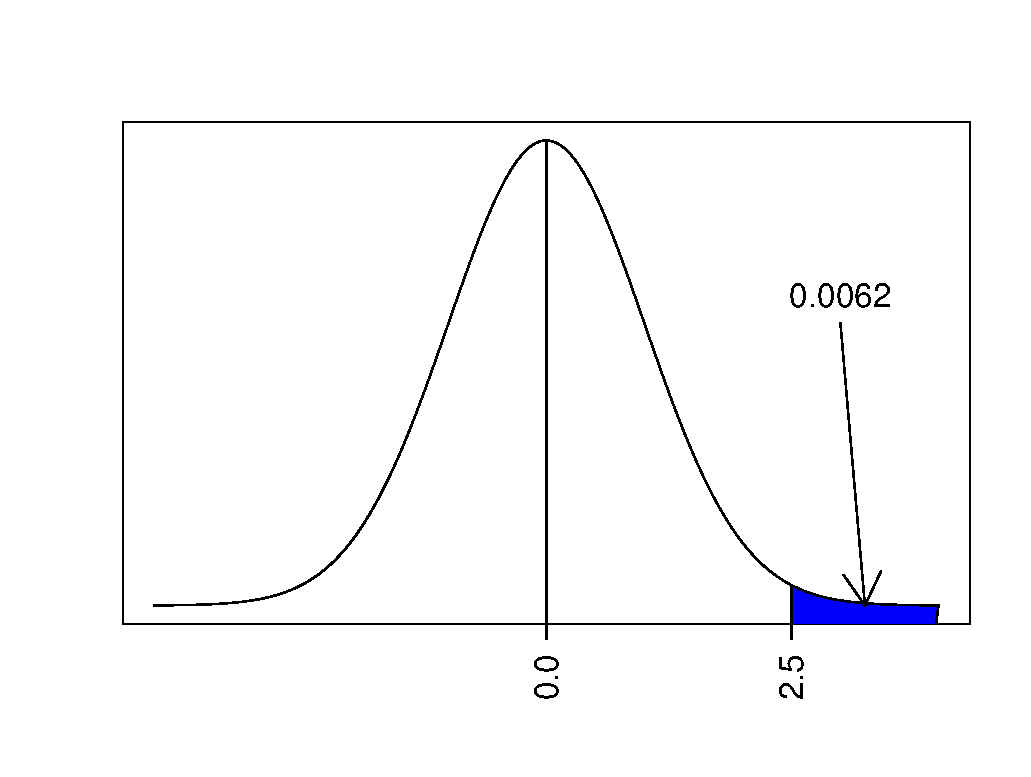
\includegraphics[scale=0.4]{gas-mileage/3a.pdf}
\end{center}
\red{$\mathrm{P}(X > 32)  = \mathrm{P}(Z > 2.5) = 1 - \mathrm{P}(Z < 2.5) = 1 - 0.9938 = 0.0062$}
\end{enumerate}

\item \textbf{[3 pts]} What is the probability a car will obtain a miles per gallon for highway driving less than 24 mpg? Answer this question by completing parts (i) and (ii). 

\begin{enumerate}
\item \textbf{[1 pt]}Provide the z-score corresponding to the above statement. \\
 \red{$z = \frac{x-\mu}{\sigma}=\frac{24-28.5}{1.4}=-3.21$}
\item \textbf{[2 pts]}Based on your answer in (i), what is the probability a car will obtain a miles per gallon for highway driving less than 24 mpg?\\
\begin{center}
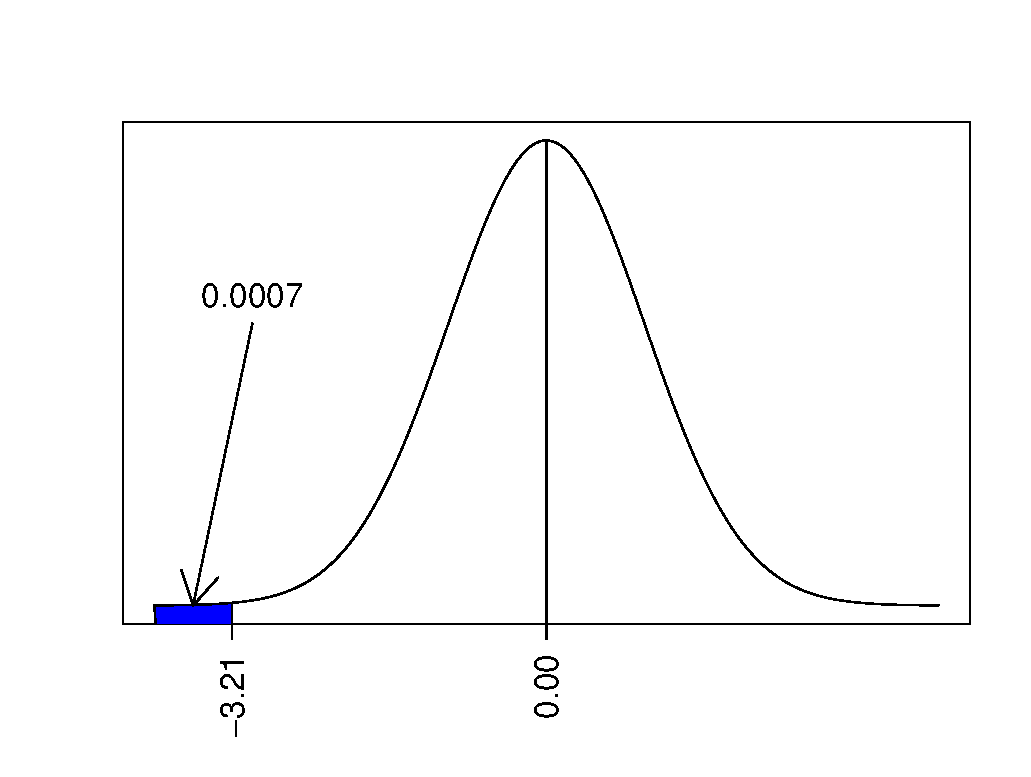
\includegraphics[scale=0.4]{gas-mileage/3b.pdf}
\end{center}
\red{$\mathrm{P}(X < 24) = \mathrm{P}(Z < -3.21) = 0.0007$}
\end{enumerate}

\newpage

\item \textbf{[3 pts]} Find $Q_1$ (First Quartile). Answer this question by completing parts (i) and (ii).  
\begin{enumerate}
\item \textbf{[1 pt]} Provide the z-score corresponding to the above statement. \\
\begin{center}
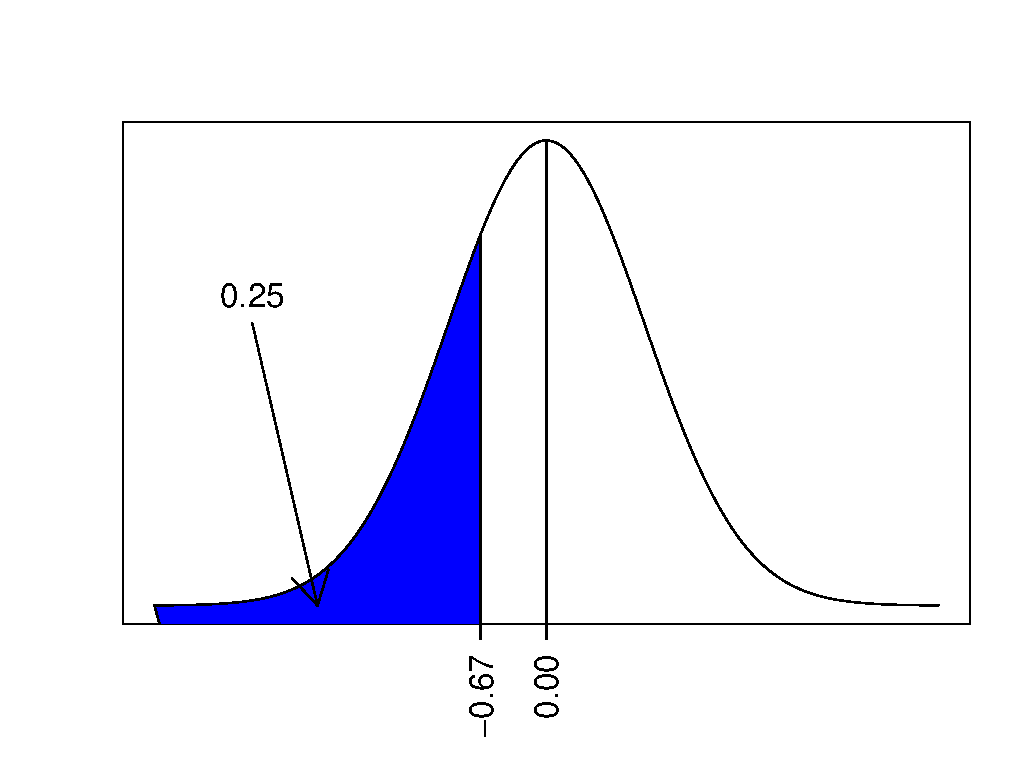
\includegraphics[scale=0.4]{gas-mileage/3c.pdf}
\end{center}
\red{$Q_1$ is the 25th percentile. For a standard normal distribution, the 25th percentile is $z = -0.67$.}
\item  \textbf{[2 pts]} Based on your answer in (i), provide the value of $Q_1$.  (Round answer to 3 decimal places.)\\
\red{The 25th percentile of X is then $Q_1 = z \times \sigma + \mu =  (-0.67)(1.4) + 28.5 = 27.562$ mpg.}
\end{enumerate}

\item \textbf{[3 pts]} Find $Q_3$ (Third Quartile). Answer this question by completing parts (i) and (ii).  

\begin{enumerate}
\item \textbf{[1 pt]} Provide the z-score corresponding to the above statement. \\
\begin{center}
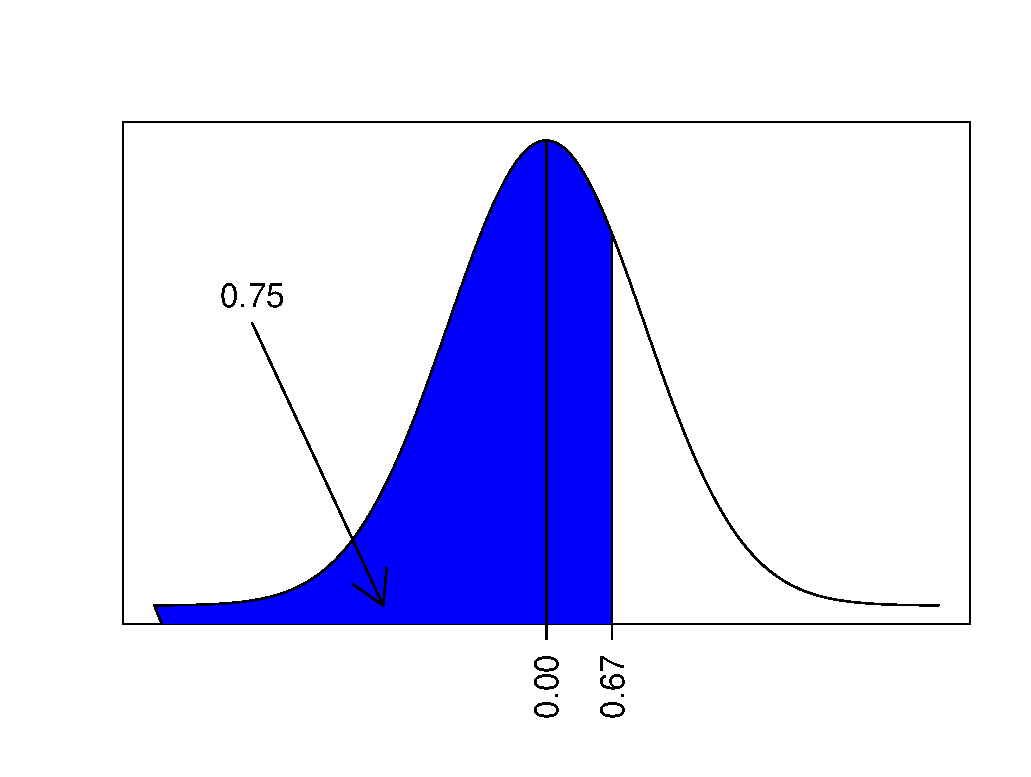
\includegraphics[scale=0.4]{gas-mileage/3d.pdf}
\end{center}
\red{$Q_3$ is the 75th percentile. For a standard normal distribution, the 75th percentile is $z = 0.67$.}
\item \textbf{[2 pts]} Based on your answer in (i), provide the value of $Q_3$.  (Round answer to 3 decimal places.)\\
\red{The 75th percentile of X is then $Q_1 = z \times \sigma + \mu =  (0.67)(1.4) + 28.5 = 29.438$ mpg.}
\end{enumerate}

\item \textbf{[1 pt]} What is the value of the IQR for the distribution of miles per gallon ratings for highway driving?  (Round answer to 3 decimal places.)\\
\red{IQR = Q3 - Q1 =29.438 - 27.562 =1.876 mpg.}

\newpage

\item \textbf{[4 pts]}What is the mpg rating such that only 4\% of all cars have an mpg rating larger than that mpg value?  Answer this question by completing parts (i) and (ii).  
\begin{enumerate}
\item \textbf{[1 pt]} Provide the z-score corresponding to the above statement. \\
\begin{center}
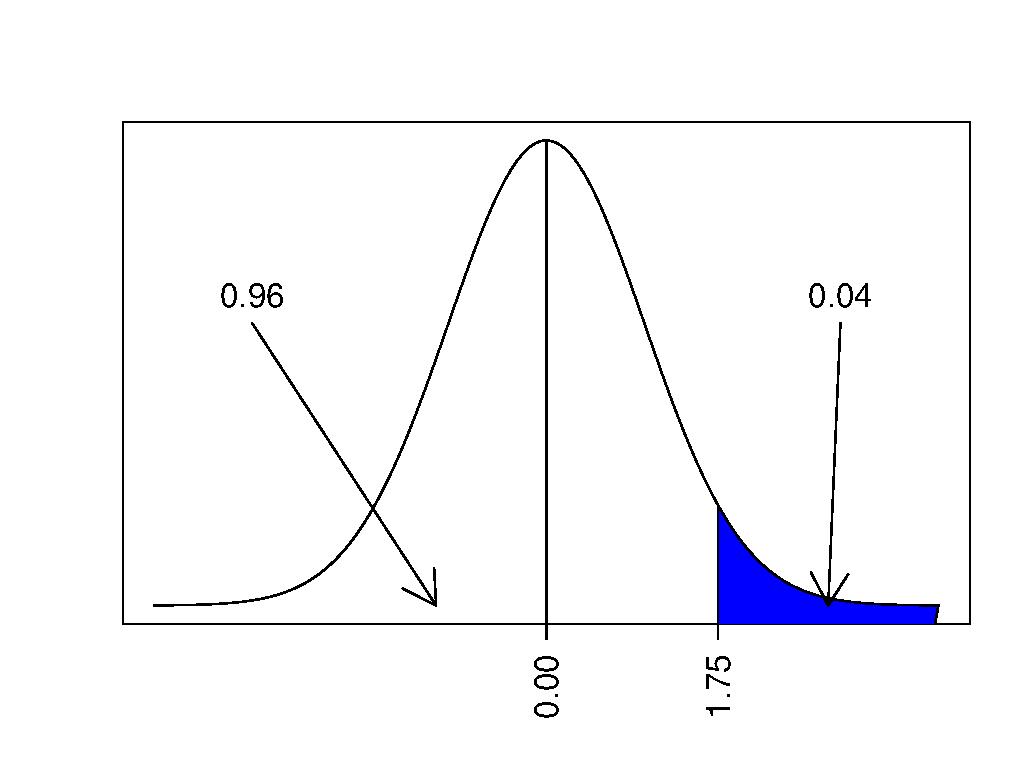
\includegraphics[scale=0.4]{gas-mileage/3f.pdf}
\end{center}
\red{The z-score with 4\% above it is the z-score with 96\% below it.  For a standard normal distribution, the z-score with 96\% below it is $z=1.75$.}
\item \textbf{[2 pts]} Based on your answer in (i), what is the mpg rating such that only 4\% of all cars have an mpg rating larger than that mpg value?  (Round answer to 2 decimal places.)\\
\red{$x = z \times \sigma + \mu =  (1.75)(1.4) + 28.5 = 30.95$ mpg.}
\item  \textbf{[1 pt]} What percentile does the mpg rating obtained in part (ii) correspond to?   (Enter value as a whole number, not a proportion.)\\
\red{The 96th percentile.}
\end{enumerate}

\item \textbf{[4 pts]} What proportion of cars will have an mpg rating within 3 mpg of the mean?  Answer this question by completing parts (i) through (iii).  
\begin{enumerate}
\item  \textbf{[1 pt]} Provide the SMALLER z-score corresponding to the above statement.\\
 \red{3 mpg below the mean is 25.5 mpg.  So, $z = \frac{x-\mu}{\sigma}=\frac{25.5-28.5}{1.4}=-2.14$}
\item  \textbf{[1 pt]} Provide the LARGER z-score corresponding to the above statement.\\
 \red{3 mpg above the mean is 31.5 mpg.  So, $z = \frac{x-\mu}{\sigma}=\frac{31.5-28.5}{1.4}=2.14$}
\item  \textbf{[2 pts]} Based on your answers in (i) and (ii), what proportion of cars will have an mpg rating within 3 mpg of the mean?\\
\begin{center}
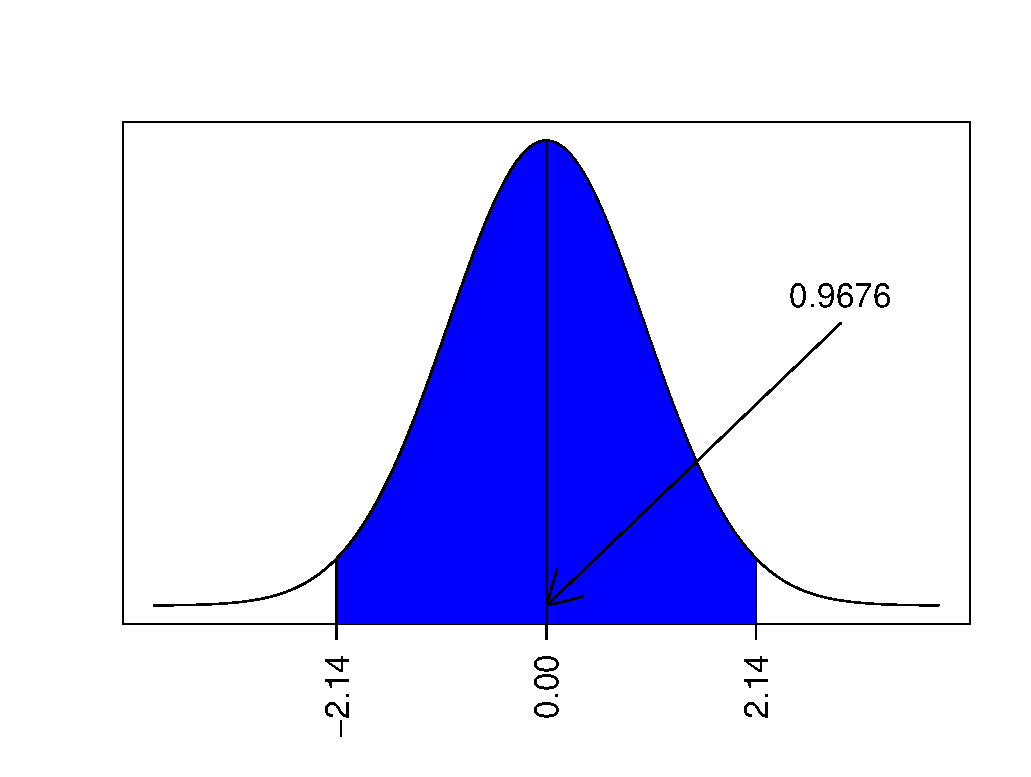
\includegraphics[scale=0.4]{gas-mileage/3g.pdf}
\end{center}
\red{$\mathrm{P}(25.5 < X < 31.5) =\mathrm{P}(-2.14 < Z < 2.14)= \mathrm{P}(Z < 2.14) -  \mathrm{P}(Z < -2.14) = 0.9838 -0.0162 = 0.9676$}
\end{enumerate}

\newpage

\item \textbf{[3 pts]} Which car is more unusual, a car with a 32 mpg rating for highway driving or a car with a 25 mpg rating for highway driving? Explain your answer. \\
\red{Both cars are equally unusual because the mpg ratings corresponding to both cars are 3.5 mpg away from the mean which is 28.5 mpg.}

\item \textbf{ [3 pts]} Let's say you bought a car of the particular model discussed in this question and extensive testing shows that you get, on average, 28.5 mpg for your car on the highway. Provide an interpretation of your car's mpg rating, i.e. what can you say about how your car compares to all other cars of this particular model?   \\
\red{Since the mean is 28.5 mpg and the mpg rating of cars is Normal, we can say that  we expect 50\% of the cars to have a lower mpg rating as compared to our car while 50\% of the cars will have a higher mpg rating compared to our car.}

\end{enumerate}